\chapter{Statistical phylogeography}

Nested clade analysis represented the earliest attempt to develop a
formal approach to using an estimate of phylogenetic relationships
among haplotypes to infer something both about the biogeographic
history of the populations in which they are contained and the
evolutionary processes associated with the pattern of diversification
implied by the phylogenetic relationships among haplotypes and their
geographic distribution. The statistical parsimony part of NCA depends
heavily on coalescent theory for calculating the ``limits'' of
parsimony. As a result, NCA combines aspects of pure phylogenetic
inference{\dash}parsimony{\dash}with aspects of pure population
genetics{\dash}coalescent theory{\dash}to develop a set of inferences
about the phylogeographic history of populations within species. But
well before NCA was developed, Pamilo and Nei~\cite{Pamilo-Nei-1988}
pointed out that the phylogenetic relationships of a single gene might
be different from those of the populations from which the samples were
collected.

\section*{Gene trees {\it versus\/} population trees}\index{gene tree}\index{population tree}

There are several reasons why {\it gene trees\/} might not match {\it
  population trees}.

\begin{itemize}

\item It could simply be a problem of estimation. Given a particular
  set of gene sequences, we {\it estimate} a phylogenetic relationship
  among them. But our estimate could be wrong. In fact, given the
  astronomical number of different trees possible with 50 or 60
  distinct sequences, it's virtually certain to be wrong somewhere. We
  just don't know where. It could be that if we had the right gene
  tree it would match the species tree.

\item There might have been a hybridization event in the past so that
  the phylogenetic history of the gene we're studying is different
  from that of the populations from which we sampled. Hybridization is
  especially likely to have a large impact if the locus for which we
  have information is uniparentally inherited, e.g., mitochondrial or
  chloroplast DNA. A single hybridization event in the distant past in
  which the maternal parent was from a different population will give
  mtDNA or cpDNA a very different phylogeny than nuclear genes that
  underwent a lot of backcrossing after the hybridization event.

\item If the ancestral population was polymorphic at the time the
  initial split occurred alleles that are more distantly related
  might, by chance, end up in the same descendant population~(see
  Figure~\ref{fig:ancestral-polymorphism})\index{ancestral polymorphism}

\end{itemize}

\begin{figure}
\begin{center}
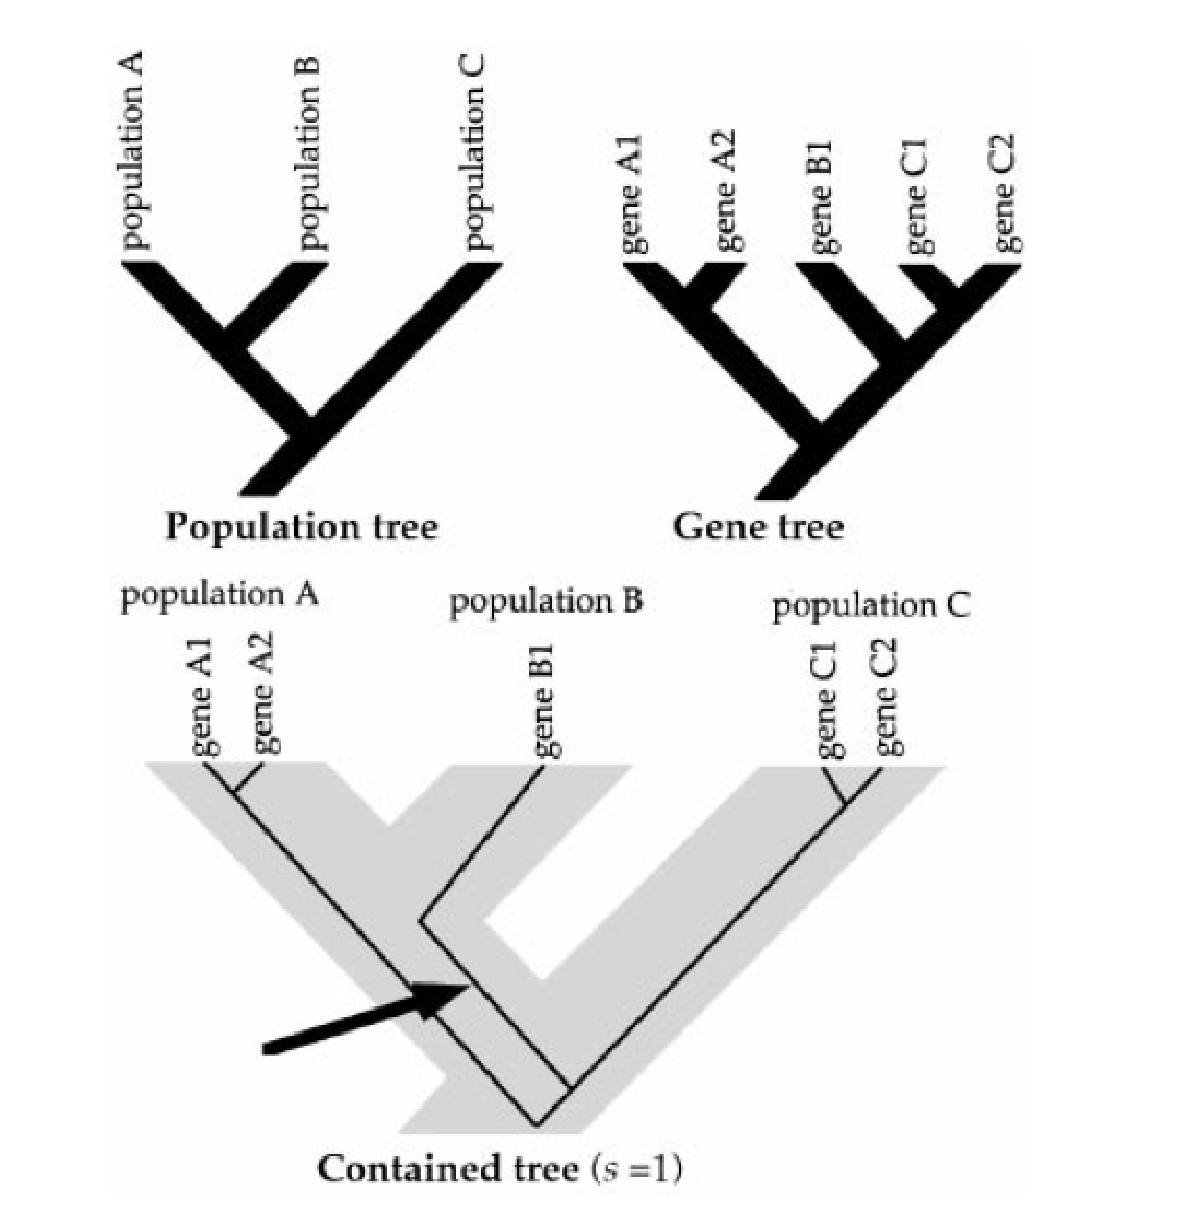
\includegraphics[height=6cm]{ancestral-polymorphism.eps}
\end{center}
\caption{Discordance between gene and population trees as a result of
  ancestral polymorphism
  (from~\cite{Knowles-2001}).}\label{fig:ancestral-polymorphism} 
\end{figure}

As Pamilo and Nei showed, it's possible to calculate the probability
of discordance between the gene tree and the population tree using
some basic ideas from coalescent theory. That leads to a further
refinement, using coalescent theory directly to examine alternative
biogeographic hypotheses.

\section*{Phylogeography of montane grasshoppers}

Lacey Knowles studied grasshoppers in the genus {\it Melanopus}. She
collected 1275bp of DNA sequence data from cytochrome oxidase I (COI)
from 124 individuals of {\it M. oregonensis\/} and two outgroup
speices. The specimens were collected from 15 ``sky-island'' sites in
the northern Rocky Mountains~(see Figure~\ref{fig:sky-islands};
\cite{Knowles-2001}). Two alternative hypotheses had been proposed to
describe the evolutionary relationships among these
grasshoppers~(refer to Figure~\ref{fig:divergence-hypotheses} for a
pictorial representation):\index{Melanopus@\textit{Melanopus}}

\begin{figure}
\begin{center}
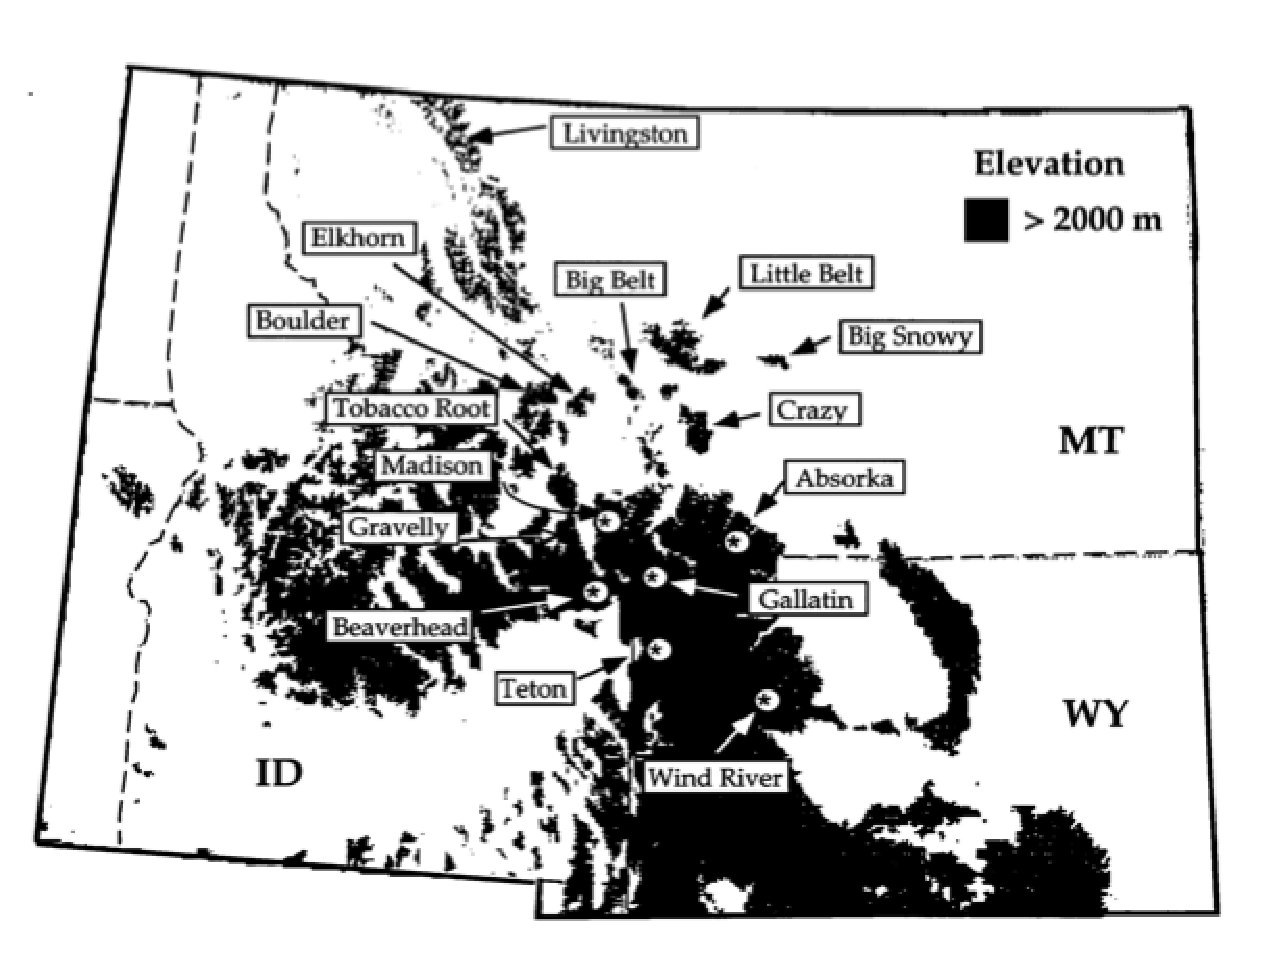
\includegraphics[height=6cm]{sky-islands.eps}
\end{center}
\caption{Collection sites for {\it Melanopus oregonensis\/} in the
  northern Rocky Mountains~(from~\cite{Knowles-2001}).}\label{fig:sky-islands}
\end{figure}

\begin{itemize}

\item {\bf Widespread ancestor}: The existing populations might represent
  independently derived remnants of a single, widespread
  population. In this case all of the populations would be equally
  related to one another.

\item {\bf Multiple glacial refugia}: Populations that shared the same
  refugium will be closely related while those that were in different
  refugia will be distantly related.

\end{itemize}

\begin{figure}
\begin{center}
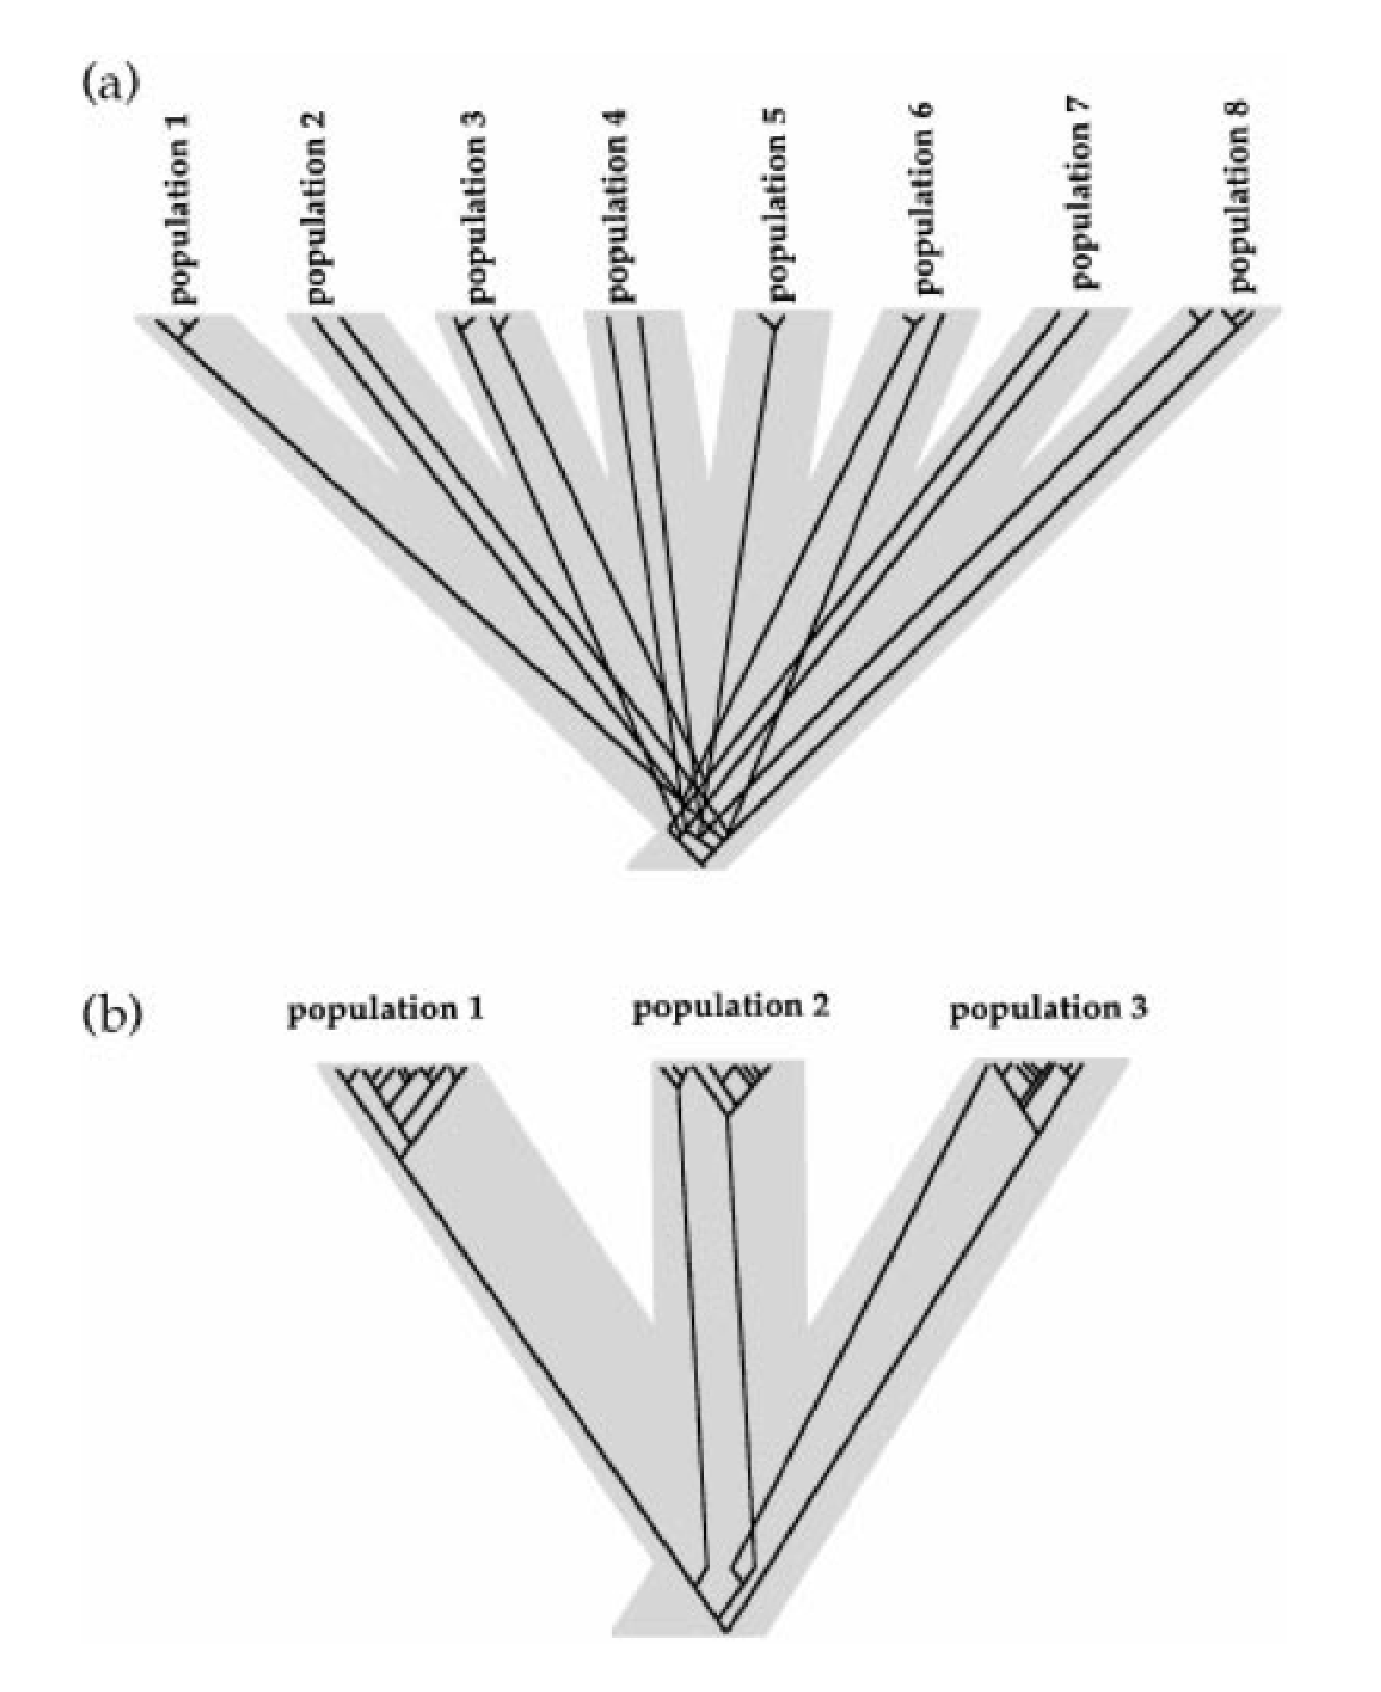
\includegraphics[height=6cm]{divergence-hypotheses.eps}
\end{center}
\caption{Pictorial representations of the ``widespread ancestor''
  (top) and ``glacial refugia'' (bottom)
  hypotheses~(from~\cite{Knowles-2001}).}\label{fig:divergence-hypotheses}
\end{figure}

As is evident from Figure~\ref{fig:divergence-hypotheses}, the two
hypotheses have very different consequences for the coalescent history
of alleles in the sample. Since the interrelationships between
divergence times and time to common ancestry differ so markedly
between the two scenarios, the pattern of sequence differences found
in relation to the geographic distribution will differ greatly between
the two scenarios. 

Using techniques described in Knowles and
Maddison~\cite{Knowles-Maddison-2002}, Knowles simulated gene trees
under the widespread ancestor hypothesis. She then placed them within
a population tree representing the multiple glacial refugia hypothesis
and calculated a statistic, $s$, that measures the discordance between
a gene tree and the population tree that contains it. This gave her a
distribution of $s$ under the widespread ancestor hypothesis. She
compared the $s$ estimated from her actual data with this distribution
and found that the observed value of $s$ was only 1/2 to 1/3 the size
of the value observed in her simulations.\footnote{The discrepancy was
  largest when divergence from the widespread ancestor was assumed to
  be very recent.} In short, Knowles presented strong evidence that
her data are not consistent with the widespread ancestor
hypothesis.\index{statistical phylogeography!example}

